\section{Задание}
Заданием данной лабораторной работы является создание модели для придуманного объекта.

В качестве моделируемого объекта была выбрана сдача лабораторных и получение зачёта. 

На зачёт приходят студенты через интервал времени $5\pm2$ минуты. Они делятся на тех, у кого сдано 0, 1 и 2 лабораторных работы. Последние сразу получают билет и становятся в очередь для ответа преподавателю. На приём одного зачёта преподаватель тратит $5\pm1$ минут, при этом есть $5\%$ вероятность того, что студент будет пойман на списывании (реальное количество списывающих студентов не уточняется), в таком случае он получает отказ и уходит без зачёта. 

Студенты, не сдавшие все лабораторные, показывают их последовательно магистрам, после чего также становятся в очередь на зачёт. На приём каждой лабораторной также создаётся по очереди. Первая лабораторная принимается одним магистром, обеспечивающим обслуживание работы за $10\pm1$. С вероятностью в $10\%$ он может найти погрешность и отправить студента доделывать лабораторную в конец своей очереди. Аналогично лабораторная №2 принимается двумя магистрами с интервалами приёма в $15\pm5$, $10\pm2$ минуты и вероятностью нахождения недочёта в $10\%$ и $20\%$ соотвественно.

Промоделировать процесс обработки 100 студентов.

\begin{figure}[h]
	\begin{center}
		{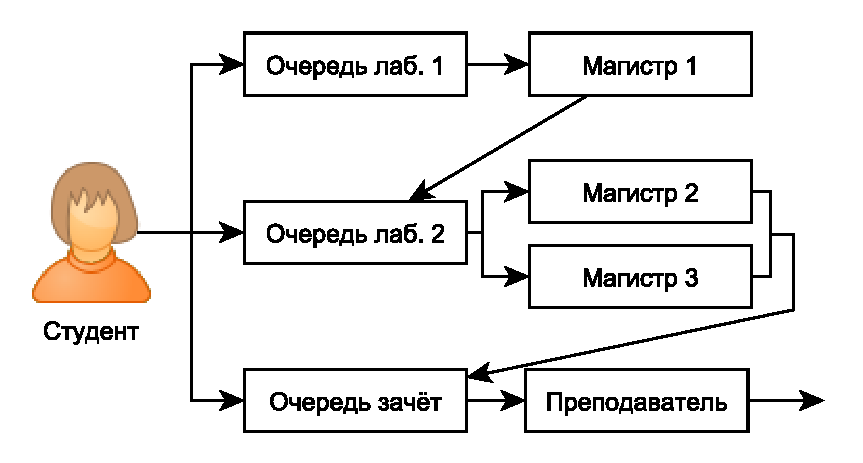
\includegraphics[scale=0.8]{kids.pdf}
			\caption{Схема модели}
			\label{pic:1}}
	\end{center}
\end{figure}